\subsection{Energiespeicher}

Die gesamte Energiespeicherung erfolgt durch einen Lithium-Ionen Akkumulator des Typs XXX. Dieser weist eine Kapazität von 800mAh bei einer Spannung von 3.7V auf. Daraus lässt sich bei einem durchschnittlichen Verbrauch von XXX W die maximale Zeit t gemäss nachfolgender Formel \ref{fig:Betriebszeit} berechnen.
\begin{equation}
t_{max}=\frac{W\cdot U}{P_{tot}}=\frac{800mAh \cdot 3.7V}{XXX W}=0.XXX h
\label{fig:Betriebszeit}
\end{equation}


Bei optimaler Bedingung und dem Schnelllademodus mit einem Strom von 400mA, ist untenstehende Abbildung  \ref{fig:Ladekurve Li-Ion Akku}  gültig. Hierbei ist ersichtlich, dass für die Spannungsregelung rund 2.5h erforderlich sind. Für die Stromregelung (letzten 20\% des Ladezyklus) noch 30 Minuten.



\begin{figure}[H]
	\begin{center}
		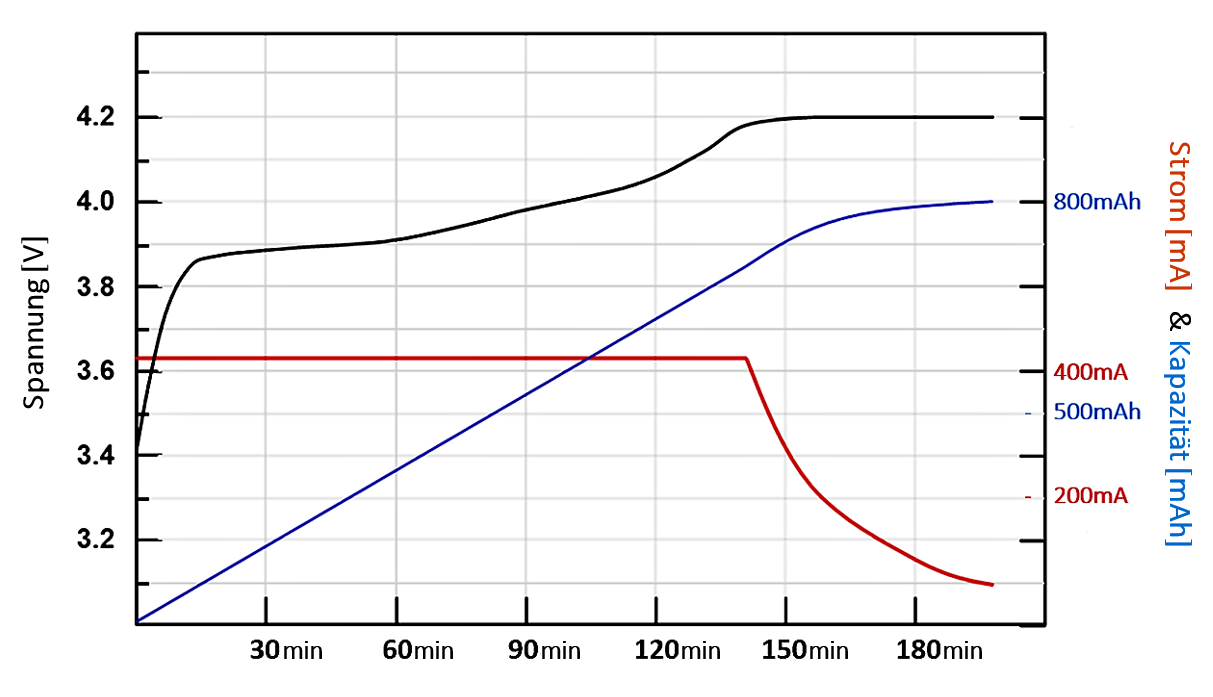
\includegraphics[width=120mm]{data/LadekurveLiIon.png}
		\caption{Blockschaltbild Energiespeicherung} %picture caption
		\label{fig:Ladekurve Li-Ion Akku}
	\end{center}
\end{figure}

%Hierbei ist gut ersichtlich, dass die letzten ca. 20\% der Aufladung auf einem Spannungslevel von 4.2V erfolgen. Für die Regelung wird ein Batterielade-IC vom Typ MCP73831T verwendet.Während dem Ladevorgang kann hierbei zusätzlich 1 LED für die Signalisation des Ladevorgangs angesteuert werden. Für die Entladeüberwachung gibt es zwei Möglichkeiten welche noch von der Batterie abhängig sind. Bei der einen Variante kann die Spannung der Batterie auf zwei Pins am Microcontroller angeschlossen und auf dem Microcontroller selber überwacht werden. Dies gewährleistet dass bei niedriger Spannung das gesamt System heruntergefahren und so der Akku vor Tiefentladung geschützt werden kann. Bei der anderen Variante weist der eingebaute Akku bereits ein Tiefentladungsschutz vor und schaltet sobald eine bestimmte Spannungsschwelle unterschritten wird die Energieversorgung ab. Da momentan noch kein 100$\%$ passender Akku gefunden wurde, bleibt es noch offen welche Variante schlussendlich realisiert wird. %

